%!TEX root = ../../../thesis.tex

Details of components in the electrode-electrolyte interface model and methods of determining its parameters have been discussed.
Research effort will now move to measuring and fitting suitable parameter values to the model.
Model parameters are determined for various concentrations of phosphate buffered saline (PBS), and then for comparison -- in a living sheep's spinal cavity.
The comparison will show whether a one-tenth concentration of PBS is in-fact a good substitute for cerebrospinal fluid (CSF), which it is assumed to be by medical implant engineers.

\section{Phosphate Buffered Saline}


    Scott \& Single fitted parameters of their model to a one-tenth concentration (0.1X) of a standard solution of PBS; a buffered saline solution \cite{Scott2014}.
    I measure and fit parameters not only to the one-tenth concentration, but to six concentrations spanning 0.025X to 1X the concentration of a standard buffered saline solution.
    For the model parameters that change with salinity, a fit is made using regression analysis to PBS concentration.
    Doing this gives a model that can be used to predict the impedance response of an electrode array submerged in a wider range of concentrations of saline solutions.

    Each of the PBS measurements were made in \SI{1000}{\milli\litre} glass bottles containing \SI{700}{\milli\litre} of the PBS solution to be measured.
    Measurements were made in a temperature controlled environment set at \SI{21}{\degree} Celsius.
    All measurements were automated by the use of Python scripts running on a GNU/Linux based workstation.
    The scripts communicate with the instruments both to configure measurements and collect data.
    Each measurement set was repeated for each of the six solutions used.
    The six concentration of PBS that were measured are shown in \cref{tab:pt2-PBS_concentrations}.
    \begin{table}
      \centering
      \begin{tabular}{l}
        Concentration\\
        \hline
        1.00X\\
        0.5X\\
        0.25X\\
        0.1X\\
        0.05X\\
        0.025X\\
      \end{tabular}
      \caption{\label{tab:pt2-PBS_concentrations}Six PBS concentrations used to fit model parameters to.}
    \end{table}


    \subsection{Inter-electrode resistivity}


      \begin{figure}
        \centering
        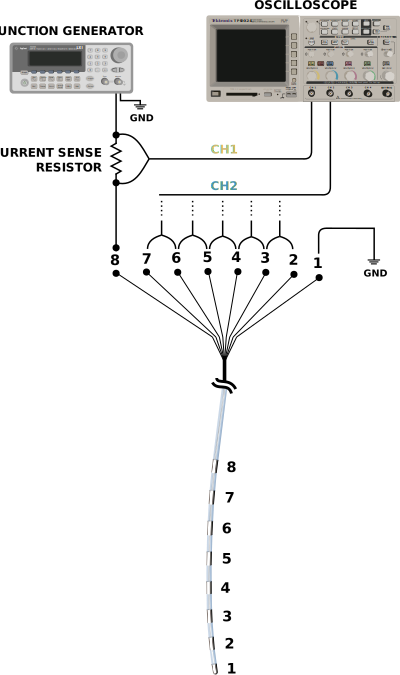
\includegraphics{content/pt2/08-InterfaceParameters/graphics/measurement_resistorMesh}
        \caption{\label{fig:pt2-measurement_resistorMesh}Illustration of one of two measurement configurations used to to measure the electrode transimpedances. Each of the electrode pairs were measured one-after-the-other using the shown equipment.}
      \end{figure}

      With the electrode array immersed in a saline solution, a \SI{10}{\kilo\hertz} sinusoidal current having a peak amplitude of \SI{500}{\micro\ampere} was passed through the stimulus electrodes using an Agilent 33220A function generator.
      A shunt resistor inserted in series with the function generator allows measurement of current between electrodes.
      The differential voltage across a pair of non-stimulating electrodes and the voltage across the shunt resistor was measured using a Tektronix TPS 2024 oscilloscope.
      \Cref{fig:pt2-measurement_resistorMesh} shows the measurement configuration used when electrodes one and eight are used as the stimulus electrodes.
      The second configuration has electrodes eight and seven as stimulus electrodes and the remaining electrode pairs are used to measure transimpedance voltage differentials.

      \begin{figure}
        \centering
        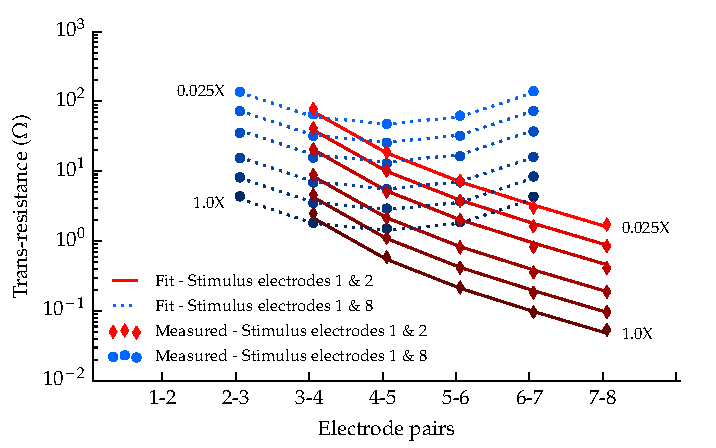
\includegraphics{content/pt2/07-InterfaceModel/graphics/graph_transimpedance_pbs}
        \caption{\label{fig:pt2-graph_transimpedance_pbs}Measured and fitted values of trans-impedance for both measurement configurations. Voltage measurements are made between adjacent pairs of electrodes as current is pushed through the stimulus electrodes.}
      \end{figure}
      The results of those measurements, in both configurations, are represented as markers in \cref{fig:pt2-graph_transimpedance_pbs}.
      Each point is calculated by taking the voltage differential across a pair of electrodes ($V_{diff}$) and dividing by the stimulus current.
      Remember, the stimulus current was set to be around \SI{500}{\micro\ampere} peak.
      \begin{table}
        \centering
        \begin{tabular}{r | l}
          Parameter & Value \\
          \hline
          $R_{eri}$ ($\Omega$)& 0.407 / $\sigma$\\
          $R_{sri}$ ($\Omega$)& $R_{eri}\cdot 3/4$\\
          $R_{li}$ ($\Omega$)& 3.71 / $\sigma$ \\
          Depth (layers) & 5 \\
          Padding (layers) & 3 \\
        \end{tabular}
        \caption{\label{tab:RESparams}Resistor mesh parameters for the electrode array in various concentrations of PBS. Electrolyte conductivity ($\sigma$) is expressed in units of $S / cm$.}
      \end{table}

      Values for $R_{eri}$ and $R_{li}$ were determined using a Python optimisation script for each concentration of PBS.
      The optimisation script selects candidate values for $R_{eri}$ and $R_{li}$, simulates the mesh using those values, and then calculates the equivalent trans-impedance values.
      The error between simulated trans-impedance values and measured values is calculated and the process repeats, selecting different values of $R_{eri}$ and $R_{li}$ to improve the fit.
      The final values of $R_{eri}$ and $R_{li}$ are those that minimise the error, they are shown in \cref{tab:RESparams}.
      $R_{sri}$ is a dependent variable, so is expressed in terms of $R_{eri}$, and the remaining parameters have been re-used from the work of Scott \& Single.
      \Cref{fig:pt2-graph_transimpedance_pbs} shows measurement results for each pair of non-stimulated pair of electrodes along with simulated results using the fitted parameters.


    \subsection{Constant phase element \& series resistance}


      \begin{figure}
        \centering
        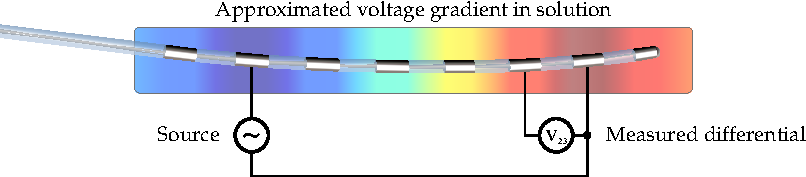
\includegraphics{content/pt2/08-InterfaceParameters/graphics/measurement_CPE}
        \caption{\label{fig:pt2-measurement_CPE}Illustrated voltage gradient in electrolyte solution at each electrode's surface when potential is applied across electrodes two and seven. Measurement of electrolyte voltage taken between electrodes 2 and 3.}
      \end{figure}
      Measurement of both the CPE and the interface's series resistance is made using an impedance spectroscopy method.
      These measurements are made by passing a sinusoidal current between electrodes two and seven of the electrode array.
      Use of the end electrodes (one and eight) was avoided as a precaution to reduce end effects resulting from the electrode's geometry.
      The sinusoidal voltage at the liquid side of the interface is taken as the the voltage that appears at an adjacent electrode (electode three) when a suitably high impedance measurement is made, this is illustrated in \cref{fig:pt2-measurement_CPE}.
      This measurement relies on the ability to make high impedance voltage measurements to minimise voltage drop across the electrode interface, for which the Tektronix TPS 2024 four channel oscilloscope was used again.
      This oscilloscope has floating channels, each having an input resistance of \SI{10}{\mega\ohm} when using 10X probes.
      The Agilent 33220A function generator was used again to generate the stimulus waveforms applied between electrodes two and eight.
      A current sense resistor of \SI{10}{\kilo\ohm} was inserted in series with the waveform generator's output and was measured by the oscilloscope.
      \begin{figure}
          \centering
          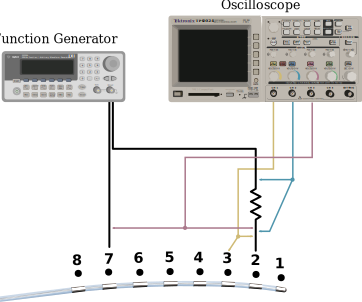
\includegraphics[scale=0.95]{content/pt2/08-InterfaceParameters/graphics/measurement_CPE_setup}
          \caption{\label{fig:pt2-measurement_CPE_setup}Diagram showing the measurement configuration used to measure the CPE response and interface series resistance.}
      \end{figure}
      By measuring the current through electrode two and the voltage across the interface (measured between electrode two and three), the impedance of the interface is calculated.
      A diagram of the measurement setup is shown as \cref{fig:pt2-measurement_CPE_setup}.
      For each of the six solutions, twenty frequencies (log-spaced) were sampled between \SI{50}{\milli\hertz} and \SI{10}{\kilo\hertz} for the impedance measurements.
      At each frequency the stimulus waveform amplitude was re-adjusted to be \SI{300}{\milli\volt}-peak as the interface's impedance changed.
      \begin{figure}
        \centering
        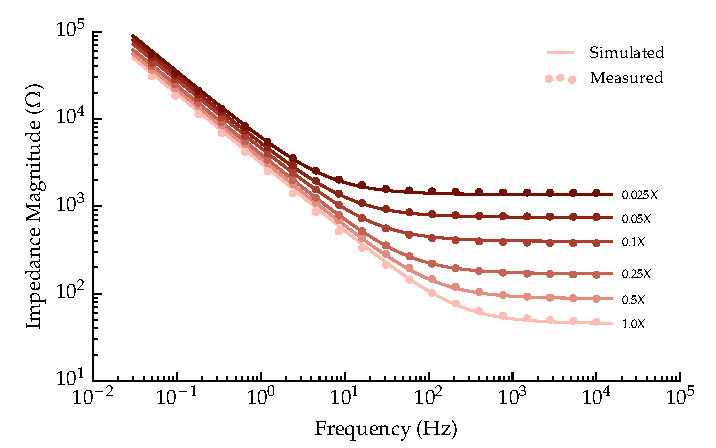
\includegraphics{content/pt2/08-InterfaceParameters/graphics/displacement_impedanceVsFrequency_magnitude_thesis}
        \caption{\label{fig:pt2-graph_impedanceVsFrequency_magnitude}Impedance magnitude of both the measured interface response and the fitted response at each of the six concentrations of PBS.}
      \end{figure}
      \begin{figure}
        \centering
        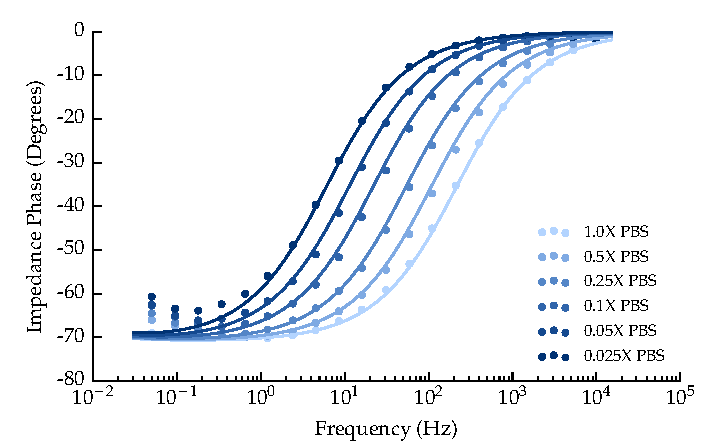
\includegraphics{content/pt2/08-InterfaceParameters/graphics/displacement_impedanceVsFrequency_phase_thesis}
        \caption{\label{fig:pt2-graph_impedanceVsFrequency_phase}Impedance phase of both the measured interface response and the fitted response at each of the six concentrations of PBS.}
      \end{figure}
      \Cref{fig:pt2-graph_impedanceVsFrequency_magnitude,fig:pt2-graph_impedanceVsFrequency_phase} show the calculated impedance magnitude and phase from measurements as markers and simulation results of the fitted parameters as traces.
      \begin{figure}
        \centering
        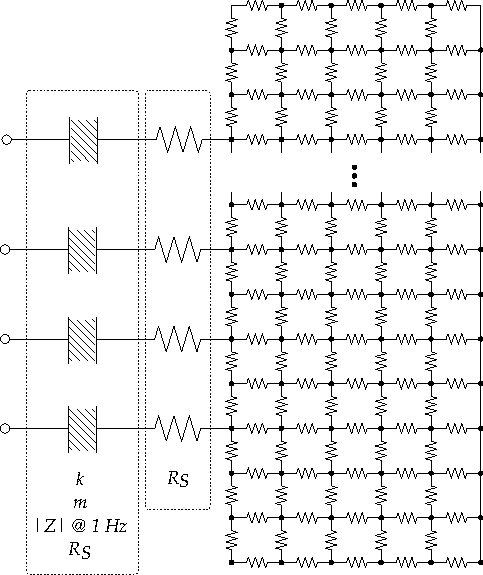
\includegraphics{content/pt2/08-InterfaceParameters/graphics/SpiceModel_opitimisation}
        \caption{\label{fig:pt2-spiceModel_optimisation}The SPICE model schematic used to find optimum values for parameters of the CPE and interface series resistance. Parameters for the resistor mesh are those determined previously.}
      \end{figure}
      \Cref{fig:pt2-spiceModel_optimisation} shows the SPICE model used to simulate parameter values for the CPE and $R_{s}$.
      Final values were found by minimising the difference between the simulated response and the measured response using a Python script.
      For each set of parameter values in the optimisation the script builds a SPICE circuit using those parameter values, simulates the circuit, calculates the interface impedance and compares the values to the measured results.
      The process is automated and runs until a minimum error between simulated and measured results is found.
      Once found, the script exists and displays the final values of each parameter.
      After parameter values are found for each concentration of PBS, another optimisation is made to scale relevant parameters by the concentration.
      The parameters that are scaled with concentration are the series resistance ($R_{S}$) and the CPE's impedance magnitude at \SI{50}{\milli\hertz}.
      The final fit expresses these parameters as functions dependent on PBS concentration (salinity).
      \begin{figure}
        \centering
        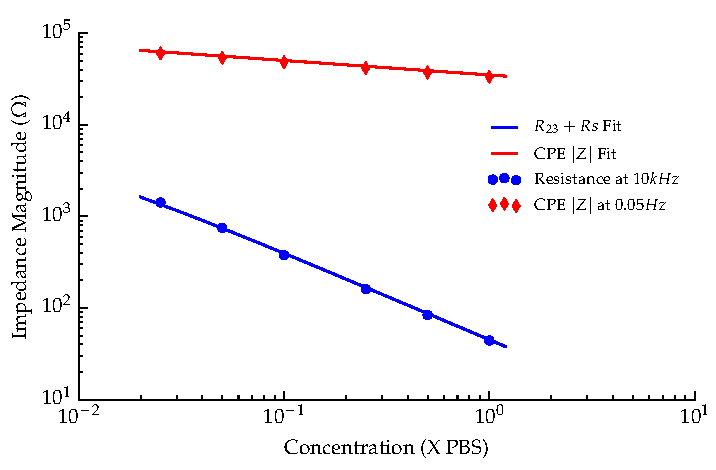
\includegraphics{content/pt2/08-InterfaceParameters/graphics/scalingFactors_Displacement_Thesis}
        \caption{\label{fig:pt2-scalingFactors_Displacement_Thesis}Plot showing fitted parameter values for the CPE impedance magnitude at \SI{50}{\milli\hertz} and series resistance at each of the six concentrations of PBS (shown as markers). The solid trace shows the resulting fit between those values as a function of concentration.}
      \end{figure}
      Individual parameter values for each concentration, along with the resulting fit, is shown in \cref{fig:pt2-scalingFactors_Displacement_Thesis}.
      Measurements of the CPE's vertical position were made at \SI{50}{\milli\hertz}, as opposed to the parameters defined value at \SI{1}{\hertz}, to avoid any effect from the series resistance interfering with the measured value.
      As the slope of the CPE is always the same, the value can be easily converted back to the equivalent value at \SI{1}{\hertz}.
      Measured resistance at high frequency includes the inter-electrode resistance ($R_{23}$) which has been included in the plot, but will be subtracted to leave only $R_{S}$.
      \begin{table}
        \centering
        \begin{tabular}{r | l}
          Parameter & Value \\
          \hline
          $m$& 1.34\\
          $k$ & 1.773\\
          |Z| @ \SI{1}{\hertz} ($\Omega$)& $3284 \times concentration^{-0.158}$ \\
          $R_{S}$ ($\Omega$)& $13.38 \times concentration^{-0.8397}$
        \end{tabular}
        \caption{\label{tab:CPEparams}CPE and $R_{s}$ parameters. Concentration is relative to the stock solution of phosphate buffered saline.}
      \end{table}
      The final parameters for the CPE and $R_{S}$ are given in \cref{tab:CPEparams}.


    \subsection{Faradaic current}


      \begin{figure}
        \centering
        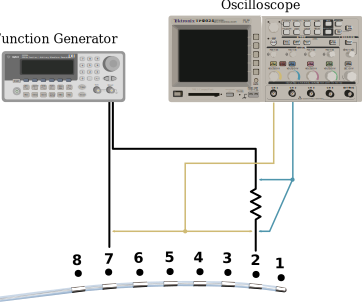
\includegraphics{content/pt2/08-InterfaceParameters/graphics/measurement_Faradaic_setup_initial}
        \caption{\label{fig:pt2-measurement_Faradaic_setup_initial}Illustration of the cyclic voltammetry measurement configuration used to measure the response of the interface when driven into Faradaic conduction mode.}
      \end{figure}
      Using the same oscilloscope and function generator as the previous measurement, the oscilloscope is set to measure voltage between electrodes two and seven and the current through the current sense resistor.
      The function generator is set to produce a triangle wave stimulus, or linear ramp, also between electrodes two and seven.
      Electrical current associated with Faradaic reactions rises exponentially after a threshold electrode overpotential.
      The point at which the electrical current draw begins to move exponentially with increasing voltage represents the onset of the associated reaction.
      \begin{figure}
        \centering
        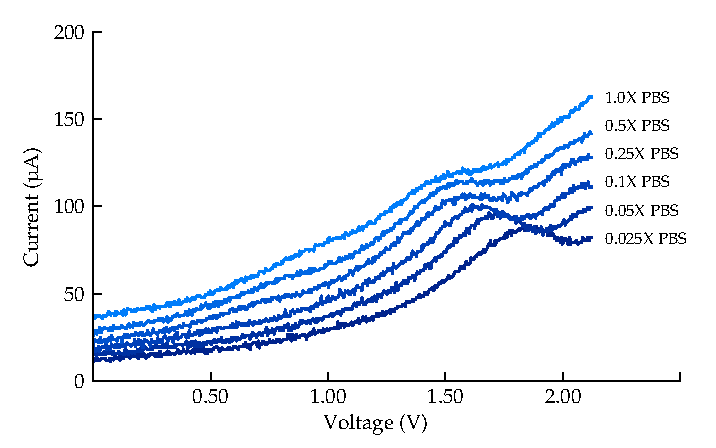
\includegraphics{content/pt2/08-InterfaceParameters/graphics/faradaicOnset-all-average}
        \caption{\label{fig:pt2-faradaic_measurement}Graph showing measured Faradaic response of each concentration of PBS to a linearly increasing voltage between electrodes two and seven.}
      \end{figure}

      \Cref{fig:pt2-faradaic_measurement} shows measured data where the Faradaic response is evident for each concentration.
      The repeatability of these measurements was low although care was taken to recreate the same conditions for each run.
      To try and improve the repeatability the following was tried:
      \begin{itemize}
        \item Maintaining a constant ambient temperature
        \item Cleaning the electrodes between each measurement using isopropyl alcohol
        \item Keeping the electrolyte moving at a constant velocity using a motorised stirrer
        \item Letting the system to settle for periods up to two hours between measurements
      \end{itemize}
      These steps reduced variation between measurements, but by no means removed the variation.
      Sweeping the voltage at \SI{0.12}{\volt\per\second} was slow enough that results did not appear to be too distorted but fast enough that a measurement run could be completed quickly.
      Completing measurements quickly seemed important at the time as it was often the case that an artifact would show up during a measurement run, for what seemed like no apparent reason, and affect the remainder of the experiments.
      Artifacts were sometimes a peak at a certain voltage, otherwise they would manifest themselves as distortions to the current/voltage trace.
      A key insight was realising that after the voltage across a pair of electrodes had been pushed into Faradaic region they then began to behave differently, even after being returned to lower stimulus voltages.
      In \cref{fig:pt2-faradaic_measurement} it is clear that each concentration has a different Faradaic response.
      This means that when the maximum voltage is applied to each of the solutions that the highest concentration is driven further into its Faradaic region that the rest.
      That in turn would create an artifact that would appear on the remaining traces (those of lower concentration), that would not have otherwise been there.
      The issue of artifact and dependence on sweep rate led me to find other ways of measuring Faradaic currents.

      \subsubsection*{Step based Faradaic measurements}
        \begin{figure}
          \centering
          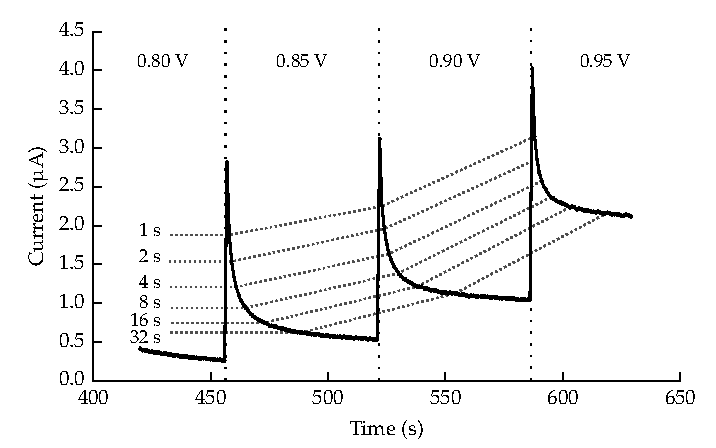
\includegraphics{content/pt2/08-InterfaceParameters/graphics/graph_64s_stirred}
          \caption{\label{fig:pt2-faradaic_decay}Graph showing measured response of two interfaces to a multiple step responses. Vertical dotted lines indicate when in time the step occurred. Dotted traces show points in time after each response. Measurements are between electrodes two and seven on the Octrode submerged in 1X PBS.}
        \end{figure}

        A revealing measurement came from the use of the Agilent E5270B precision measurement mainframe, the same instrument that was used to measure the streaming potential cells of \cref{part:doubleLayersOnInsulators}.
        By increasing the voltage between the electrodes in discrete steps and recording the current over time it became clear that the CPE was having a large effect on the Faradaic measurements.
        \Cref{fig:pt2-faradaic_decay} shows three transitions in steps of \SI{50}{\milli\volt} occurring \SI{64}{\second} apart.
        The dotted traces show what the result would be if the measurement were taken at that time, i.e. the trace would take the shape of the dotted line of the corresponding delay time.
        This graph shows the effect the CPE is having on measurement results, as well as the duration of time necessary for the transient response to settle in most instances.

        \begin{figure}
          \centering
          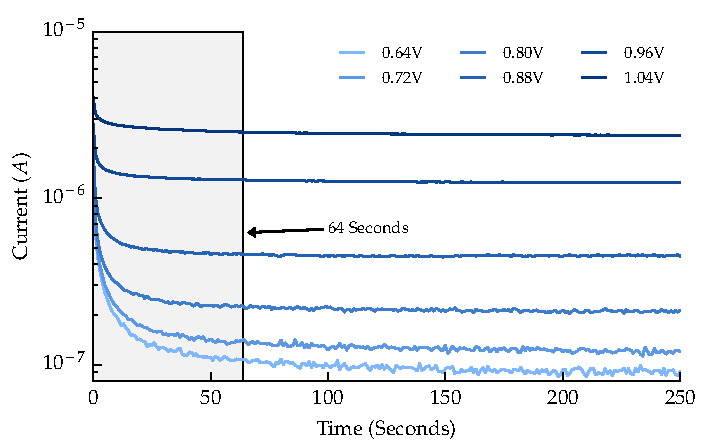
\includegraphics{content/pt2/08-InterfaceParameters/graphics/graph_CPE_currentVsTime_thesis}
          \caption{\label{fig:graph_CPE_currentVsTime}Graph showing CPE discharge curve after a step transition between each of voltage trace in increasing order. Measurements are between electrodes two and seven on the Octrode submerged in 1X PBS. A delay of 10 000 seconds elapsed between each step.}
        \end{figure}
        Subsequent measurements of CPE settling time show that a delay of \SI{64}{\second} between steps is adequate to allow the CPE voltage to settle.
        These measurements are shown as \cref{fig:graph_CPE_currentVsTime}, with the \SI{64}{\second} window highlighted in grey.
        It is interesting to note from these measurements that the capacitance appears to be a function of the applied overpotential, with lower potentials resulting in larger capacitance.

        \begin{figure}
          \centering
          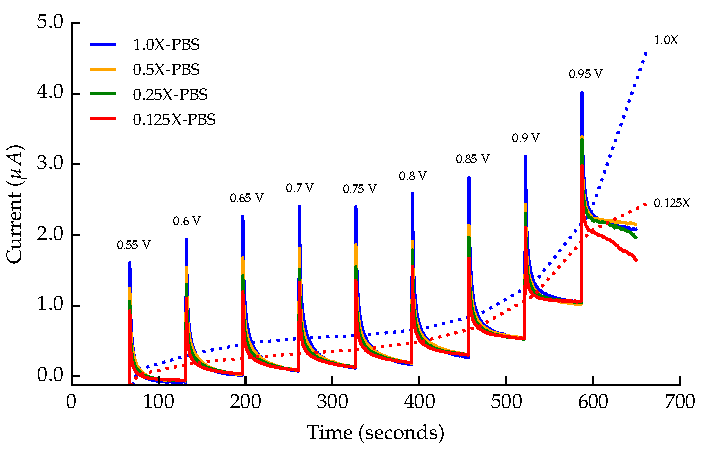
\includegraphics{content/pt2/08-InterfaceParameters/graphics/graph_currentTimeFaradaicCPE_Stacked_Thesis}
          \caption{\label{fig:graph_currentTimeFaradaicCPE_Stacked_Thesis}Graph showing measurements of four concentrations of PBS as each is stepped from \SI{0.55}{\volt} to \SI{0.95}{\volt}. Measurements are between electrodes two and seven on the Octrode. A delay of 64 seconds elapsed between each step. Dotted traces connect current measurements taken \SI{10}{\second} after each step.}
        \end{figure}
        \Cref{fig:graph_currentTimeFaradaicCPE_Stacked_Thesis} shows measurements of four concentrations of PBS overliad on top of one another.
        This graph reveals that not only does the capacitance vary with applied voltage, as was shown in \cref{fig:graph_CPE_currentVsTime}, but also with concentration of PBS.
        A consequence of this is that not waiting long enough to sample the current gives the impression that a higher concentration of PBS results in larger Faradaic currents.
        This is shown by the dotted trace that is sampled \SI{10}{\second} after each step, which I believe is representative of results obtained using cyclic voltammetry methods.
        Importantly -- the settled current draw for each concentration is the same.
        Any separation between concentrations at the sixty-four second mark for each step appear to be completely random.

        \subsubsection*{Successful measurement of the Faradaic current}
        \begin{figure}
          \centering
          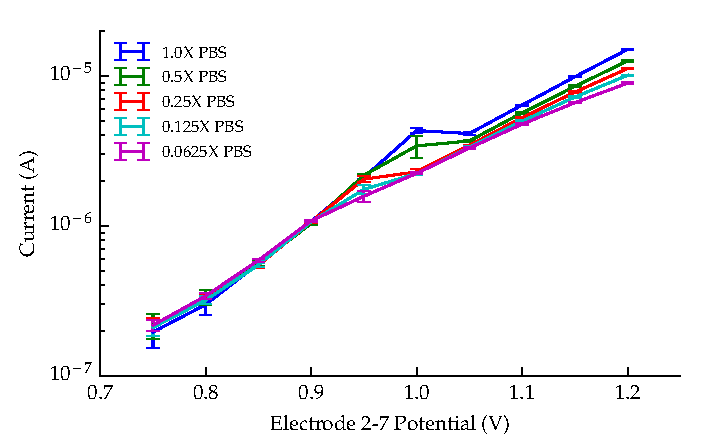
\includegraphics{content/pt2/08-InterfaceParameters/graphics/graph_currentVoltage_logY_Thesis}
          \caption{\label{fig:graph_currentVoltage_logY_Thesis}Graph showing the electrical current draw associated with Faradaic reactions versus applied electrode overpotential. Measurements used the stepped method with a wait time of \SI{64}{\second} between transitions. Vertical bars mark the standard deviation of the final fourty measurements before the following step.}
        \end{figure}
        \Cref{fig:graph_currentVoltage_logY_Thesis} shows the collected measurements of the electrical current due to Faradaic reactions using the stepped measurement method.
        Spread in the measurements at low voltages is due to noise in the measurement samples.
        There are three important observations that can be made from this graph:
        \begin{enumerate}
          \item The effect saline concentration below \SI{0.9}{\volt} has little to no significance on the Faradaic current draw.
          \item Saline concentration is directly related to Faradaic current draw above \SI{1.05}{\volt}.
          \item Between \SI{0.9}{\volt} and \SI{1.05}{\volt} each trace transitions to a mode of saline concentration dependence in reverse order of saline concentration.
        \end{enumerate}

        It appears that the change in behavior between \SI{0.9}{\volt} and \SI{1.05}{\volt} is due to a transition to diffusion-controlled conduction between electrodes.
        I hypothesise that below \SI{0.9}{\volt} the charging of the CPE draws available ions to the electrode, creating a layer of high ionic concentration at the surface irrespective of that of the solution bulk.
        It is this layer that is consumed by the Faradaic reactions at a rate that increases exponentially with electrode overpotential.
        The effect of the bulk solution concentration while this layer exists is negligible until the point at which the layer is consumed faster than it can be replenished.
        At this point, and with increasing overpotential, Faradaic conduction is governed by diffusion of ions from the solution bulk into that layer.
        The rate at which those new ions diffuse into the layer is a function of the concentration, or abundance of ions available in the bulk.
        I believe this explains the divergence of conduction with concentration between \SI{0.9}{\volt} and \SI{1.05}{\volt} and why there is no observable dependence on the bulk ion concentration beforehand.
        As Faradaic reactions are dangerous in an implanted setting, and therefore to be avoided, interest in Faradaic reactions lies in determining their onset.
        For the purpose of model it is sufficient to place a \SI{0.9}{\volt} limit across a pair of electrodes and proceed on the basis that Faradaic conduction is not affected by the saline concentration.

        \begin{figure}
          \centering
          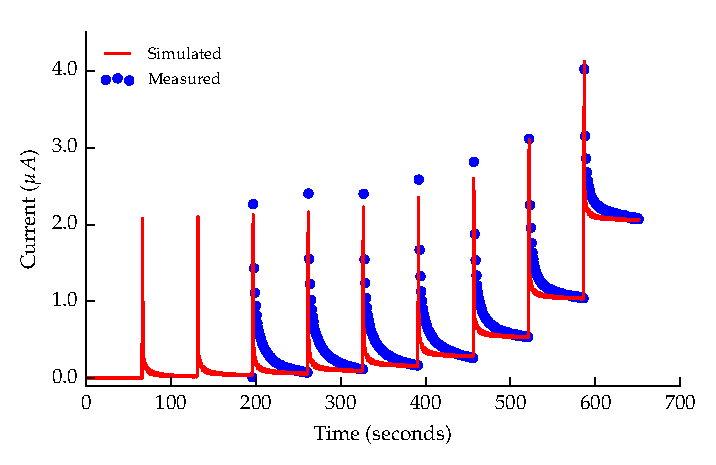
\includegraphics{content/pt2/08-InterfaceParameters/graphics/graph_faradaic_currentVsTimeThesis}
          \caption{\label{fig:graph_faradaic_currentVsTimeThesis} Graph comparing measured Faradaic response of a pair of interfaces (1.0X PBS) to the simultated response using fitted parameter values for $i_0$ and $n$. Each spike is a step in electrode overpotential, with the steps shown in the following graph.} 
        \end{figure}
        \begin{figure}
          \centering
          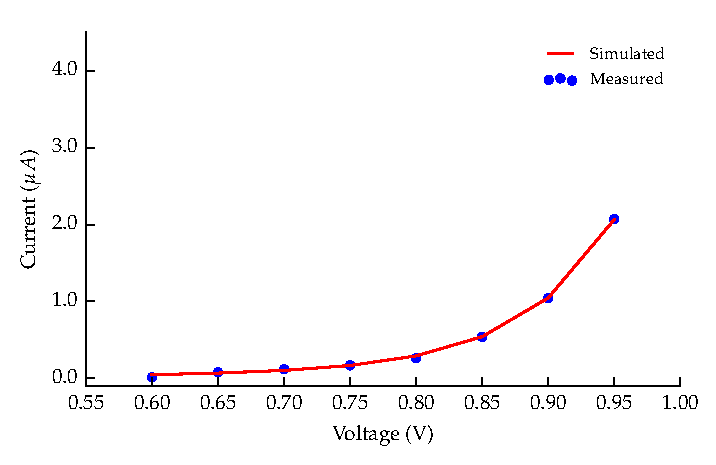
\includegraphics{content/pt2/08-InterfaceParameters/graphics/graph_faradaic_currentVsVoltageThesis}
          \caption{\label{fig:graph_faradaic_currentVsVoltageThesis} Graph comparing the measured settled electrical currents of Faradaic reactions (in 1.0X PBS) for a pair of interfaces to simulated final values using the fitted parameter values for $i_0$ and $n$.}
        \end{figure}
        Using the ``step and wait'' method to measure electrical currents associated with Faradaic conduction gave improved results, both in repeatability and expected response.
        \Cref{fig:graph_faradaic_currentVsTimeThesis,fig:graph_faradaic_currentVsVoltageThesis} show results using the 1.0X PBS solution; the other concentrations followed the same pattern.
        In \cref{fig:graph_faradaic_currentVsTimeThesis} it can be seen that the simulated CPE does not follow the decay curve of the interface after each transition.
        Notice again how the rate of decay appears to be dependent on the electrode overpotential, with higher voltages resulting in lower apparent capacitance.
        This suggests that in order for the simulated CPE to better represent the interface's displacement characteristics it should also take the electrode overpotential as a parameter to modify its behavior.
        No effort was made to incorporate the scaling of capacitance into the CPE of the model, but doing so would be a valuable improvement on the current model.
        Final parameter values for the Faradaic currents (the diodes of the model) are given in \cref{tab:FaradaicParams}.

        \begin{table}
          \caption{Faradaic parameters}
          \label{tab:FaradaicParams}
          \begin{center}
            \begin{tabular}{r | l}
                Parameter & Value \\
                \hline
                $i0$ & $2.757\thinspace pA$\\
                $n$ & 1.36\\
            \end{tabular}
          \end{center}
        \end{table}


      % TODO: Write this up in an Appendix
      % \begin{figure}
      %   \centering
      %   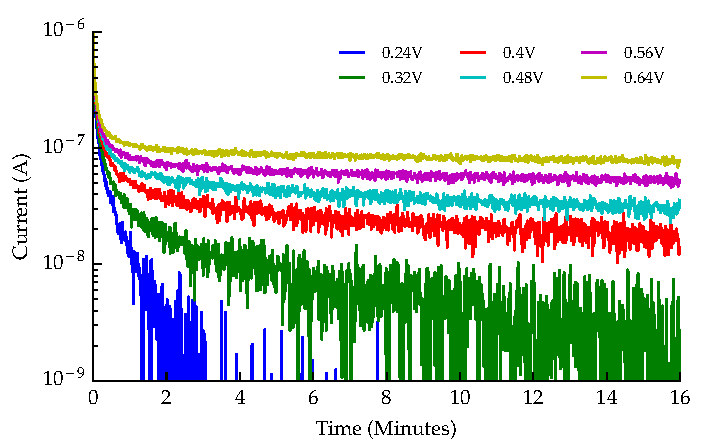
\includegraphics{content/pt2/08-InterfaceParameters/graphics/graph_longsweep_CPE}
      %   \caption{\label{fig:graph_longsweep_CPE}Graph showing current between two electrodes after the voltage is stepped to each of the shown voltages. The total settling time between transition was \SI{10000}{\second}.}
      % \end{figure}


    \subsection{Final model}


      Parameter values for each of the model's components have been found.
      Collecting the parameters that describe the interface's impedance results in \cref{tab:ModelParameters}.
      This table excludes the parameters of the resistor network as they do not describe the interface itself.

      \begin{table}
        \caption{Table of determined interface parameters for the St. Jude Medical Octrode in PBS.}
        \label{tab:ModelParameters}
        \begin{center}
          \begin{tabular}{r | l}
              Parameter & Value \\
              \hline

              $R_{S}$ ($\Omega$)& $13.38 \times concentration^{-0.8397}$ \\
              
              $m$& 1.34\\
              $k$ & 1.773\\
              |Z| @ \SI{1}{\hertz} ($\Omega$)& $3284 \times concentration^{-0.158}$ \\

              $i0$ & $2.757\thinspace pA$\\
              $n$ & 1.36\\
          \end{tabular}
        \end{center}
      \end{table}

      \begin{figure}
        \centering
        
\includegraphics{content/pt2/08-InterfaceParameters/graphics/interfaceSchematic_PBS_Solved}
        \caption{\label{fig:interfaceSchematic_PBS_Solved} Schematic of the electrode-electrolyte interface including parameter values for platinum and buffered saline.}
      \end{figure}


\section{Epidural Insertion in Live Sheep}
  \label{sect:sheep_measurements}


  \begin{figure}
    \centering
    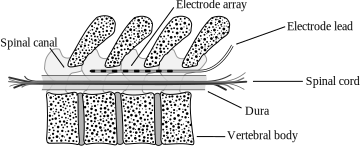
\includegraphics{content/pt2/08-InterfaceParameters/graphics/sheepSpine}
    \caption{\label{fig:sheepSpine} Diagram showing the positioning of the St. Jude Medical Octrode electrode array inside the sheep spinal cavity.}
  \end{figure}

  The previous section dealt with measuring and fitting numerical values to the electrode-interface parameters in various solutions of buffered saline, or PBS.
  Buffered saline, specifically a 0.1X concentration of a standard saline solution, was used for electrode characterisation as it was believed to be a good substitute for cerebrospinal fluid.
  Electronic engineers at Saluda Medical used these 0.1X PBS solutions to test their implant devices to make sure they were capable of driving and handling the impedance presented by the electrode-electolyte interface and spinal cavity.
  Not knowing how closely the saline solutions resembled live biological spinal fluid they also tested their implants and electrodes in living sheep.
  A sheep's spinal canal is smaller than a human's, but large enough to insert an epidural electrode array, making them a relatively accessible means of in-vivo testing for medical applications.
  Measurement in a live sheep's spinal canal still requires a lot of resources such as a surgeon, access to an operating theater, equipment suitable for use in an operating theater, ethical approval, and time.
  In each case the test sheep would be anethesatised and kept alive for the duration of the experiments, which often lasted over twelve hours.
  A veterinary surgeon would prepare and monitor the sheep constantly during the expriments to ensure that it was fully anethatised and then euthenise the sheep at the end of testing.

  These tests offered an opportunity for me to characterise the electrode-electrolyte interface inside a living mammal.
  This section repeats the measurements and parameter value determination of the previous section but this time inside a living sheep's spinal cavity.
  The same electrode as was used in the previous measurements (St. Jude Medical Octrode) was inserted into the spinal cavity of the sheep (just outside the dura) for each experiment, as shown in \cref{fig:sheepSpine}.

  The two sheep used to gather experimental data used here were provided by the Keams Facility at the Royal North Shore Hospital of Sydney under the Animal Care and Ethics Committee approval.
  These experiments complied with the Australian Code of Practice for the Care and Use of Animals for Scientific Purposes.
  In each case the sheep were injected with alfaxalone to induce anesthesia and were then intubated and ventilated with an oxygen-air mixture containing isoflurane.
  During the course of experimentation the animals were monitored using electrocardiogram, arterial blood pressure, arterial saturation, and end-tidal (exhaled) carbon dioxide levels.
  In short, they were completely unaware of the experiments being carried out and being terminated on completion meant they never became aware.
  All ethical considerations and procedures around animal testing were handled by Saluda Medical.
  Unless otherwise stated, measurement procedures and the equipment used in the hospital are the same as those used to measure the response in PBS.

  \subsection{Inter-electrode resistivity}
  
    Transimpedance measurements were made first once the electrode array was inserted into the spinal canal.
    These measurements were more extensive than those made in saline as additional stimulus electrode pairs were used.
    The extra measurements were made with the hope that they may capture more information regarding the impedance structure of the surrounding spine geometry, namely bone.
  
    \begin{figure}
      \centering
      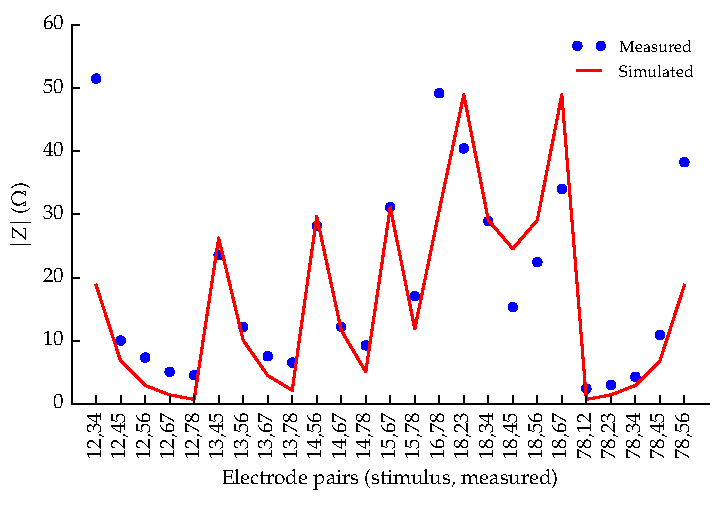
\includegraphics{content/pt2/08-InterfaceParameters/graphics/sheep_transimpedance_doubleFit_mag_thesis}
      \caption{\label{fig:sheep_transimpedance_doubleFit_mag} Graph showing measured and simulated impedance magnitude for twenty five combinations of stimulus-measure pairs of electrodes.}
    \end{figure}
  
    \begin{figure}
      \centering
      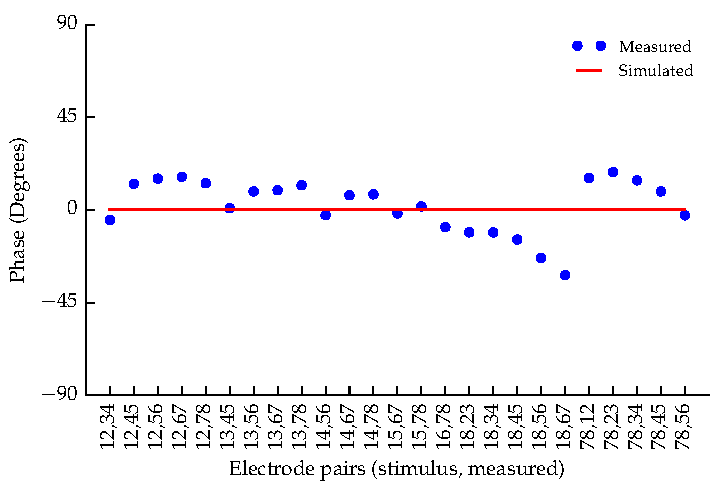
\includegraphics{content/pt2/08-InterfaceParameters/graphics/sheep_transimpedance_doubleFit_phase_thesis}
      \caption{\label{fig:sheep_transimpedance_doubleFit_phase} Graph showing measured and simulated impedance phase for twenty five combinations of stimulus-measure pairs of electrodes.}
    \end{figure}
  
    \Cref{fig:sheep_transimpedance_doubleFit_mag,fig:sheep_transimpedance_doubleFit_phase} show both the measured and simulated results for the impedance magnitude and phase response respectively.
    The magnitude measurements show that when stiumlating between electrodes one and eight and measuring on electrodes two and three that the impedance is approximately that of the one-tenth concentration of PBS (compared with results from \cref{fig:pt2-graph_transimpedance_pbs}).
    This result adds validation to the notion that the one-tenth concentration of a standard buffered saline solution is a good substitute for a spinal cavity.
    For the case where the stimulus is placed between electrode one and two and the impedance is measured between electrodes seven and eight, comparison points toward a lower concentration of PBS.
    Swapping the stimulus and measure electrodes around gave different trans-impedance values, i.e., the point at 12,78 does not equal that of 78,12.
    It is most probably a result of the electrode array shifting whilst inside the sheep, for which nothing could have been done to prevent.
  
    One important insight from these measurements is the phase response, as is shown in \cref{fig:sheep_transimpedance_doubleFit_phase}.
    As much as 30 degrees of phase angle between the stimulus current and electrode voltage was observed when separation between the stimulus and measure pairs is at its maximum.
    This shows that the spinal cavity itself is a significantly reactive component.
    For comparison, the PBS solutions displayed no measurable reactance for all of the equivalent trans-impedance measurements.
    The decreasing phase angle of measurements using one and eight as stimulus electrodes is a result of the measured pair of electrodes being between the stimulus, i.e., it is a result of our electrode choices.
    There are other instances where the phase angle appears to drop below zero, but these are likely an artifact of the measurements themselves.
    Those situations only occur when the stimulus and measured electrodes are adjacent to one another and therefore the impedance, and therefore signal-to-noise ratio, was at its lowest.
    Stimulus current was reduced for the in-vivo measurements to prevent triggering of any muscles.
  
    \begin{table}
      \centering
      \begin{tabular}{r | l}
        Parameter & Value \\
        \hline
        $R_{eri}$ ($\Omega$)& 500\\
        $R_{sri}$ ($\Omega$)& 375\\
        $R_{li}$ ($\Omega$)& 176\\
        Depth (layers) & 5 \\
        Padding (layers) & 3 \\
      \end{tabular}
      \caption{\label{tab:RESparams_sheep} Table of determined resistor mesh parameters for an electrode array in a live sheep's spinal cavity.}
    \end{table}
    The simulated results shown in \cref{fig:sheep_transimpedance_doubleFit_mag,fig:sheep_transimpedance_doubleFit_phase} (shown as the red trace) were calculated using the resistor mesh parameter values shown in \cref{tab:RESparams_sheep}.
    Those values were determined using the same SciPy optimisation library for Python as was used to fit the values in PBS.
  
  
  \subsection{Constant phase \& series resistance}

    \begin{figure}
      \centering
      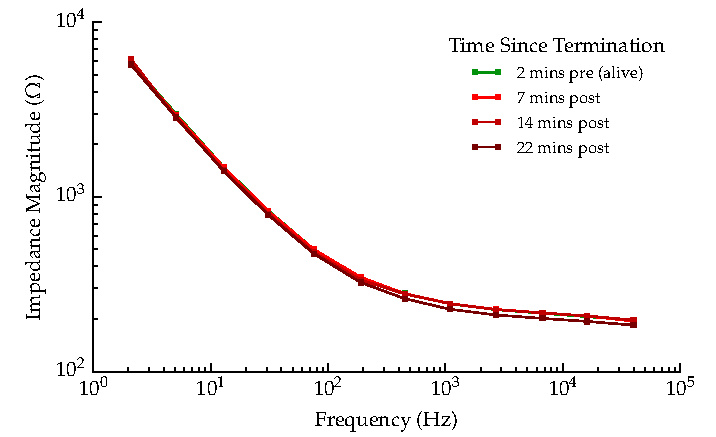
\includegraphics{content/pt2/08-InterfaceParameters/graphics/graph_Day2_Sheep_CPE_ImpedanceMagnitude}
      \caption{\label{fig:graph_Day2_Sheep_CPE_ImpedanceMagnitude} Graph showing measured CPE impedance magnitude response before and after termination.} 
    \end{figure}
    
    \begin{figure}
      \centering
      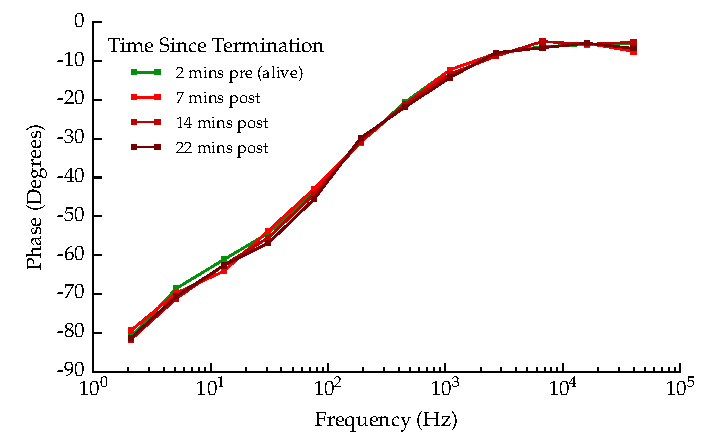
\includegraphics{content/pt2/08-InterfaceParameters/graphics/graph_Day2_Sheep_CPE_ImpedancePhase}
      \caption{\label{fig:graph_Day2_Sheep_CPE_ImpedancePhase} Graph showing measured CPE impedance phase response before and after termination.} 
    \end{figure}
  
  
    \Cref{fig:graph_Day2_sheep_CPE_ImpedanceMagnitude,fig:graph_Day2_Sheep_CPE_ImpedancePhase} shows the impedance magnitude and phase response of the CPE at the interface between the electrode and the sheep's spinal cavity.
    Reliability issues on day one meant that no useful data was captured from the first sheep, hence these figures show data only from the second sheep.
    Measurements on the second day were made over a thirty minute period starting two minutes before termination.
    
    An important question that we wished to answer was whether the impedance response in live sheep would be any different to that of a dead sheep.
    Results indicate that there is practically no difference for at least thirty minutes after termination.
    However, measurements should have been carried out over a longer time-frame after termination as it would likely take longer for the fluid composition to change.
    As the measurements required termination of the sheep, they had to be done after all other experiments had been completed.
    Since each sheep was shared between other research groups, this meant that termination happened late (early the following morning) due to accumulated delays in previous experiments.
    Measuring the CPE response in the spinal cavity of a butchered sheep would offer a useful reference point for those measurements.
    
  
    \begin{figure}
      \centering
      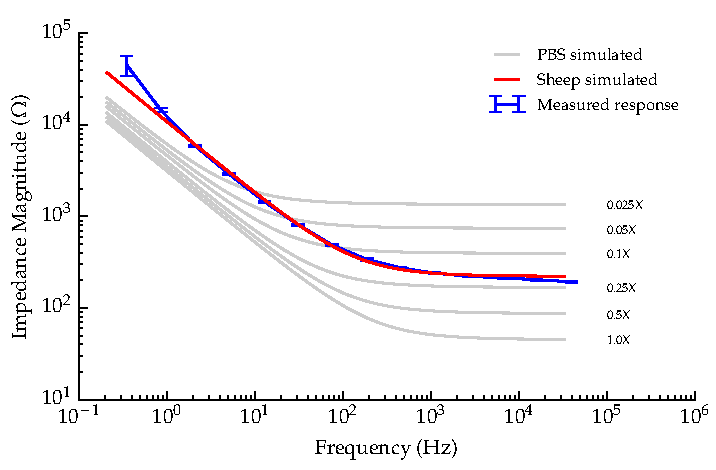
\includegraphics{content/pt2/08-InterfaceParameters/graphics/graph_displacement-withSheep_impedanceVsFrequency_magnitude_thesis}
      \caption{\label{fig:graph_displacement-withSheep_impedanceVsFrequensy_magnitude} Graph showing average CPE response in live sheep compared to the six solutions of PBS, visible as the grey traces, and simulated response based on fitted parameters.} 
    \end{figure}
    
    \begin{figure}
      \centering
      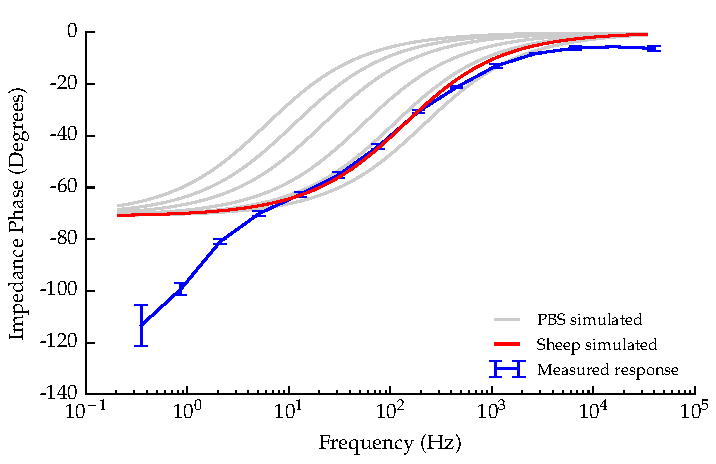
\includegraphics{content/pt2/08-InterfaceParameters/graphics/graph_displacement-withSheep_impedanceVsFrequency_phase_thesis}
      \caption{\label{fig:graph_displacement-withSheep_impedanceVsFrequency_phase} Graph showing average CPE response in a live sheep's spinal cavity compared to six concentrations of PBS, visible as grey traces, and simulated response based on fitted parameters.} 
    \end{figure}
  
    \Cref{fig:graph_displacement-withSheep_impedanceVsFrequensy_magnitude,fig:graph_displacement-withSheep_impedanceVsFrequency_phase} compares the average impedance (both magnitude and phase) of the previous graphs with the six concentrations of PBS used in the previous section.
    Simulated results from a numerical fit to the measured data appear as the red trace.
    At low frequencies, below \SI{1}{\hertz}, the simulated data deviates substantially from measured results.
    The cause for this is unclear, but in \cref{chap:fluid_mimicry} the opposite response appears when using unbuffered saline solutions - which may provide a clue.
    What is interesting is the series resistance in sheep spine is similar to that of a 0.25X PBS solution, whereas the CPE behaves more like that of a concentration much lower than 0.025X.
    Based on this data, a one-tenth concentration of PBS does appear to be a reasonable approximation to the electrolyte found in a mammalian spinal column, although the match is poor.
    In the following section the possibility of creating a solution that better matches these results will be explored.
 

  \subsection{Faradaic current}
  
    Faradaic measurements on the live animal were abandoned as they were deemed likely to cause muscle contractions.
    Attempts were made to measure Faradaic response using a much lower stimulus current but this only resulted in noise and were discarded.
    These measurements may be possible if done after a long enough duration post-termination, to prevent muscle movement.
  
  \subsection{Final model}

    \begin{table}
      \caption{Table of determined interface parameters for an electrode array in a live sheep's spinal cavity.}
      \label{tab:ModelParameters_sheep}
      \begin{center}
        \begin{tabular}{r | l}
            Parameter & Value \\
            \hline
    
            $R_{S}$ & \SI{126}{\ohm} \\
            
            $m$& 1.34\\
            $k$ & 1.77\\
            |Z| @ \SI{1}{\hertz} ($\Omega$)& \SI{11.3}{\kilo\ohm} \\
    
            $i0$ & Undetermined\\
            $n$ & Undetermined\\
        \end{tabular}
      \end{center}
    \end{table}
    Parameter values for the final sheep model are presented in \cref{tab:ModelParameters_sheep}.
    Unfortunately, the diode/Faradaic parameters were not obtained on live sheep due to safety concerns.
    Those measurements are likely to be of value to implant designers as they provide a reference for the beginnings of Faradaic conduction.
    Access to an recently terminated sheep's spine, and a surgeon, would provide a way of collecting those Faradaic measurements and additional post-termination samples.
    
    Parameters for the interface model in sheep have been fitted.
    It appears as though buffered saline, of any concentration, is not an ideal representation of a live sheep's spinal cavity.
    The next research question is to determine if it is possible to create a solution that better matches those impedance characteristics.



    
